\documentclass{CUP-JNL-DAP}%

%%%% Packages
\usepackage{graphicx}
\usepackage{amsmath,amssymb,amsfonts}
\usepackage{booktabs}
\usepackage{tabularx}
\usepackage[authoryear]{natbib}
\usepackage[T1]{fontenc}%
\usepackage{times}%
\usepackage{newtxmath}%
\usepackage{textcomp}%
\usepackage{xcolor}
\usepackage{hyperref}
%%%%

\articletype{DATA PAPER}
\jname{Data \& Policy}
\jyear{2026}
\raggedbottom

\begin{document}

\begin{Frontmatter}

\title[Physician accessibility measures for Virginia and the NCR]{Physician accessibility measures for Virginia and the National Capital Region at the census block group level}

\author*[1]{Aaron D. Schroeder}\email{ads7fg@virginia.edu}

\authormark{Aaron D. Schroeder}

\address*[1]{\orgdiv{Social Data Commons, Biocomplexity Institute and Initiative}, \orgname{University of Virginia}, \orgaddress{\city{Charlottesville}, \state{VA}, \country{USA}}}

\keywords{physician accessibility; floating catchment area; spatial analysis; Virginia; National Capital Region; open data; CMS; primary care; obstetrics; pediatrics}

\abstract{Three open-access datasets are described that measure spatial accessibility to primary care physicians, obstetrician-gynecologists (OB-GYNs), and pediatricians across Virginia and the National Capital Region (Virginia, Washington DC, and Maryland). The datasets span 2018 to 2025 for primary care and pediatric physicians and 2017 to 2025 for OB-GYNs, covering approximately 5,963 block groups, 2,198 census tracts, 133 counties, and 35 health districts. For each specialty, six measures are provided: provider count within a catchment area, mean and median travel time to the ten nearest providers, and three floating catchment area (FCA) scores (2SFCA, E2SFCA, and 3SFCA). The FCA methods account for both travel distance and population demand, using specialty-appropriate denominators: total population for primary care, females aged 15 and older for OB-GYNs, and children aged 0 to 17 for pediatricians. Provider locations are drawn from the Centers for Medicare and Medicaid Services Doctors and Clinicians public use file, population denominators from the American Community Survey, and drive times from the OpenStreetMap road network via OSRM. A shared computational pipeline produces all three FCA variants simultaneously for each specialty, yielding approximately 2.09 million records standardized to 2020 census geographies. The datasets are deposited on Zenodo under open-access licenses with source code available on GitHub. They currently supply the Virginia Public Health Data and National Capital Region community health dashboards.}

\begin{policy}
State and local health agencies allocate resources to reduce gaps in physician access, yet most available data describe provider supply only at the county level, obscuring disparities within counties. These datasets measure how easily residents of each census block group can reach primary care physicians, OB-GYNs, and pediatricians by car, updated annually from 2017 or 2018 through 2025. The accessibility scores account for both travel time and competition from nearby populations, revealing underserved areas that simple provider counts miss. Health departments, regional planning commissions, and legislatures can use these data to target workforce recruitment, site new clinics, evaluate Certificate of Public Need applications, and track whether access disparities narrow or widen over time.
\end{policy}

\end{Frontmatter}

%% ============================================================
%% INTRODUCTION
%% ============================================================

\section{Introduction}

\subsection{Policy context}

The United States faces a persistent and worsening shortage of physicians. The Association of American Medical Colleges projects a shortfall of 13,500 to 86,000 physicians by 2036, with primary care alone accounting for 20,200 to 40,400 of the deficit~\citep{aamc2024}. Recent HRSA projections place the broader physician shortage at 124,180 to 187,130 by the 2027 to 2037 period, with the most acute gaps concentrated in nonmetropolitan areas~\citep{adashi2025}. These aggregate figures obscure a structural problem: physician supply has never been evenly distributed across geographies, and the resulting maldistribution has proven resistant to decades of policy intervention~\citep{rosenthal2005}. Rural communities and low-income urban neighborhoods face systematically fewer physicians per capita, longer travel distances to care, and measurably worse health outcomes~\citep{douthit2015}.

Higher primary care supply at the state and county level is associated with lower all-cause mortality, reduced infant mortality, and fewer preventable hospitalizations~\citep{starfield2005}. In obstetric care, counties classified as maternity care deserts exhibit maternal mortality rates of 32.25 per 100,000 live births compared to 23.62 in counties with adequate access~\citep{atwani2025}. The March of Dimes estimates that half of all US counties now qualify as maternity care deserts, affecting 6.9 million women of childbearing age~\citep{marchofdimes2024}. For children, 29.6 percent of school districts lack any child-serving physician, a deficit linked to lower educational attainment as well as delayed preventive care~\citep{drescher2023}. In Virginia specifically, workforce analyses have documented shortages across primary care, nursing, and behavioral health that constrain the state's capacity to deliver equitable care~\citep{andrew2024}. The Appalachian region of the state faces 12 percent fewer primary care physicians and 65 percent fewer specialty physicians relative to national averages~\citep{marshall2017}.

Federal designation systems attempt to identify underserved areas. The Health Resources and Services Administration maintains over 8,100 primary care Health Professional Shortage Areas (HPSAs), covering roughly 100 million Americans~\citep{hrsa2024}. The National Health Service Corps, which uses HPSA designations to place clinicians, currently supports approximately 25,000 providers in shortage areas~\citep{crs2023}. These designations inform billions of dollars in federal resource allocation each year, yet the underlying data infrastructure on which they rest has significant limitations.

\subsection{Why spatial and granular data matters}

\citet{penchansky1981} defined five dimensions of healthcare access: availability, accessibility, accommodation, affordability, and acceptability. Most federal shortage metrics address only availability, measured as a provider-to-population ratio within a bounded geographic unit. This approach treats administrative boundaries as impermeable barriers, ignoring the fact that patients routinely cross county and state lines to reach care. It also collapses the spatial dimension of access, treating a county where most residents live within ten minutes of a physician identically to one where comparable ratios mask hour-long drive times for rural populations at the periphery. \citet{guagliardo2004} documented how simple ratio measures fail to capture the spatial interaction between provider locations and population concentrations, particularly in heterogeneous urban-suburban-rural regions. Block group and census tract level measurement, combined with travel time modeling, can reveal pockets of low access that county-level ratios render invisible~\citep{xia2019}. For policy instruments such as HPSA designations, Medicaid reimbursement adjustments, and residency placement incentives, the spatial resolution of the underlying data directly determines whether resources reach the populations most in need.

\subsection{Existing data resources and approaches}

A substantial body of work has applied spatial accessibility methods to physician distribution. The two-step floating catchment area (2SFCA) method, introduced by \citet{luo2003}, established the standard gravity-based framework for measuring spatial access to healthcare. The method assigns each population location an accessibility score based on the supply-to-demand ratios of all providers within a defined travel time threshold. \citet{luo2009} extended this framework with distance-decay weights (E2SFCA) to differentiate between providers at different travel distances, and \citet{wan2012} added selection weights to account for competition among providers for the same population (3SFCA). A systematic review by \citet{saxena2023} catalogued 43 methodological developments and 346 applications of gravity-based accessibility measures, confirming the FCA family as the dominant approach in health geography.

Several national and regional studies have applied these methods to physician access in the United States. \citet{xia2019} used National Plan and Provider Enumeration System (NPPES) data to compute variable-distance E2SFCA scores for primary care providers across all US ZIP codes, demonstrating that spatial accessibility patterns differ meaningfully by provider type. \citet{buchalter2025} applied multi-modal accessibility measures at the census tract and block group level using CMS quarterly data, finding that rural access disparities worsen over time. \citet{guagliardo2004b} examined pediatric provider accessibility in the District of Columbia, identifying racial and socioeconomic disparities that county-level measures failed to detect. \citet{koschinsky2024} computed drive-time measures to obstetric hospitals to map maternity care deserts at fine spatial resolution. \citet{kang2020} demonstrated reproducible E2SFCA computation using CyberGIS infrastructure for accessibility analysis in Chicago. Outside the United States, \citet{daras2019} published open accessibility data for health services across Great Britain, establishing a model for transparent, reusable spatial access datasets in the public health domain.

\citet{mcgrail2009} highlighted a persistent tension in FCA implementations: the choice of catchment size, distance-decay function, and competition weights substantially affects results, yet most studies report a single methodological variant for a single provider type, making it difficult for users to assess sensitivity to these choices.

\subsection{Methodological and data gaps}

Despite the volume of FCA research, several gaps limit the utility of existing datasets for policy analysis and monitoring. First, most published studies are cross-sectional, reporting accessibility scores for a single year. Workforce shortages and provider mobility create temporal dynamics that single-year snapshots cannot capture~\citep{buchalter2025}. Second, the majority of studies focus on a single provider type, typically primary care, making it difficult to compare access patterns across specialties that serve distinct populations with different spatial behaviors~\citep{xia2019}. Third, few studies publish their accessibility scores as reusable datasets; results typically appear as maps or summary statistics within journal articles, requiring other researchers to replicate the entire pipeline to obtain comparable data~\citep{saxena2023,daras2019}. Fourth, methodological choices (2SFCA versus E2SFCA versus 3SFCA, catchment radius, decay function) are rarely presented side by side, leaving users unable to assess how sensitive conclusions are to model specification~\citep{saxena2023,mcgrail2009}. Fifth, geographic coverage in the published literature tends toward either national analyses at coarse resolution (ZIP code or county) or highly localized case studies of individual metropolitan areas~\citep{guagliardo2004,xia2019,kang2020}. State and megaregional scales, which correspond to the jurisdictions where health workforce policy is actually enacted, remain underrepresented. \citet{gentili2018} documented pediatric primary care access disparities and accessibility gaps for publicly insured children, but noted the difficulty of producing consistent, multi-year spatial access measures suitable for tracking policy outcomes over time.

\subsection{Dataset introduction}

This paper describes three physician accessibility datasets covering Virginia and the National Capital Region (the District of Columbia and adjacent counties in Maryland and Virginia). The datasets measure spatial access to primary care physicians (family practice, family medicine, and general practice), obstetrician-gynecologists, and pediatricians at the census block group level. Primary care and pediatric datasets span 2018 to 2025; the OB-GYN dataset spans 2017 to 2025. All three datasets are produced by a shared floating catchment area pipeline that computes six measures for each block group and year: the count of providers within the catchment, mean and median travel time to the ten nearest providers, and accessibility scores from the 2SFCA~\citep{luo2003}, E2SFCA~\citep{luo2009}, and 3SFCA~\citep{wan2012} methods. Provider locations are drawn from the CMS Doctors and Clinicians public use file. Population denominators are sourced from the American Community Survey at the block group level: total population for primary care, female population aged 15 and older for OB-GYN, and population aged 0 to 17 for pediatrics. Travel times between block group centroids and provider locations are computed using the Open Source Routing Machine. All outputs use 2020 Census geographies and follow a standardized long-format schema with columns for geographic identifier, year, measure name, value, margin of error, and data method.

\subsection{Reuse value}

The datasets are designed for three categories of reuse. For health workforce policy, the multi-year time series enables tracking of access trends in response to provider recruitment programs, residency expansions, and HPSA redesignation~\citep{hrsa2024,crs2023}. State agencies and regional planning bodies can identify block groups where access has deteriorated or improved, at a resolution that aligns with the catchment areas of individual clinics and practices. For methodological research, the simultaneous provision of 2SFCA, E2SFCA, and 3SFCA scores allows direct comparison of how model choice affects accessibility rankings and the identification of underserved areas~\citep{luo2003,luo2009,wan2012,saxena2023}. Researchers can assess whether policy conclusions are sensitive to the gravity model specification without replicating the full computational pipeline. For cross-domain analysis, the standardized schema and census-aligned geographies allow direct linkage to demographic, economic, educational, and environmental datasets at the block group level~\citep{drescher2023,andrew2024,daras2019}. The inclusion of three provider types serving distinct demographic subpopulations (total population, women of reproductive age, children) supports intersectional analyses of how access varies across specialty, geography, and time.

%% ============================================================
%% METHODS
%% ============================================================

\section{Methods}

\subsection{Input data sources}

The datasets described in this paper were produced from four primary input sources. Table~\ref{tab:sources} summarizes each source, its provider, spatial resolution, and temporal coverage.

\begin{table}[ht]
\centering
\caption{Input data sources.}
\label{tab:sources}
\footnotesize
\begin{tabularx}{\textwidth}{XXlX}
\toprule
Source & Provider & Resolution & Temporal coverage \\
\midrule
Doctors and Clinicians National Downloadable File & CMS & Provider address & 2017--2025 (annual) \\
ACS 5-Year Estimates, Table B01001 & U.S. Census Bureau & Block group & 2016--2023 \\
Pre-computed travel time matrices & OpenStreetMap / OSRM v5.27.1 & BG centroid & 2020 road network \\
County-to-Health-District Crosswalk & Virginia Dept. of Health & County & 2020 \\
\bottomrule
\end{tabularx}
\end{table}

The study area encompasses two overlapping regions: the Commonwealth of Virginia (FIPS 51, all counties and independent cities) and the National Capital Region (NCR). The NCR includes nine Virginia jurisdictions (Fairfax County, Fairfax City, Falls Church, Loudoun County, Arlington County, Alexandria, Manassas, Manassas Park, and Prince William County), four Maryland counties (Frederick, Montgomery, Prince George's, and Charles), and the District of Columbia.

\subsection{Data acquisition}

\subsubsection{CMS provider data}

Provider records were obtained from the CMS Doctors and Clinicians National Downloadable File, a publicly available registry of clinicians enrolled in Medicare. Annual ZIP archives were downloaded programmatically from the CMS Provider Data website (\url{https://data.cms.gov/provider-data/dataset/mj5m-pzi6}) for each year in the study period. Each archive contains a single CSV file listing all enrolled clinicians nationwide.

The pipeline extracted the CSV from each archive, filtered records to providers with practice addresses in Virginia, Maryland, or the District of Columbia, and retained only those holding MD or DO credentials. Column names were standardized across years because CMS changed its schema multiple times during the study period (e.g., \texttt{lst\_nm} in early files, \texttt{Last Name} in intermediate files, and \texttt{Provider Last Name} in later files). After standardization, providers were filtered by specialty. Three specialty-specific datasets were constructed:

\begin{itemize}
\item \textbf{Primary care}: providers listing Family Practice, Family Medicine, or General Practice as a primary or secondary specialty (2018--2025).
\item \textbf{OB-GYN}: providers listing Obstetrics/Gynecology as a primary or secondary specialty (2017--2025).
\item \textbf{Pediatric}: providers listing Pediatric Medicine as a primary or secondary specialty (2018--2025).
\end{itemize}

Each provider was identified by a unique National Provider Identifier (NPI). Per-year filtered CSVs were saved to enable incremental updates without re-downloading the full national file.

\subsubsection{Population denominator data}

Block-group-level population denominators were drawn from the American Community Survey (ACS) 5-Year Estimates, Table B01001 (Sex by Age), retrieved through the Census Bureau API. Each specialty used a denominator appropriate to its target population:

\begin{itemize}
\item \textbf{Primary care}: total population (variable B01001\_001).
\item \textbf{OB-GYN}: female population aged 15 and older, constructed by summing 20 age-sex bins (variables B01001\_030 through B01001\_049).
\item \textbf{Pediatric}: population aged 0 to 17, constructed by summing 8 age-sex bins covering males and females under 5, 5 to 9, 10 to 14, and 15 to 17 (variables B01001\_003 through B01001\_006 and B01001\_027 through B01001\_030).
\end{itemize}

Population data were retrieved for all block groups in Virginia (FIPS 51), Maryland (FIPS 24), and the District of Columbia (FIPS 11). Because ACS 5-Year Estimates are released with a two-year lag, each CMS data year $t$ was paired with the ACS vintage $t - 1$, capped at 2023 (the latest available vintage at the time of processing). For example, CMS year 2025 used ACS year 2023.

\subsubsection{Travel time matrices}

Travel times between block group centroids were drawn from pre-computed matrices generated using the Open Source Routing Machine (OSRM) v5.27.1. OSRM was configured with the OpenStreetMap road network as of 2020, using automobile routing under free-flow conditions (no real-time traffic adjustment). Block group centroids were derived from 2020 TIGER/Line shapefiles published by the Census Bureau. Travel time matrices were stored as Apache Parquet files, one per state FIPS code, covering Virginia and all neighboring states (FIPS codes 10, 11, 21, 24, 37, 47, 51, 54) to ensure border-crossing routes were available. Each file contains origin block group, destination block group, and travel time in minutes. Pairs without a viable road route were absent from the file and treated as unreachable (assigned a cost of $10^{6}$ minutes) during matrix construction.

\subsection{Geocoding and spatial assignment}

Provider addresses were geocoded using the U.S. Census Bureau Geocoder API (Public\_AR\_Current benchmark, Current\_Current vintage). Each unique address was submitted as a single-line query. The geocoding results were cached so that addresses appearing in multiple years or across specialty datasets were geocoded only once. Successfully geocoded addresses received latitude and longitude coordinates.

Each geocoded provider address was then assigned to the nearest 2020 census block group centroid using the haversine distance formula. Provider capacity at each block group was defined as the count of unique NPIs at addresses assigned to that block group. This aggregation step collapsed multiple providers at the same physical location (e.g., a multi-physician practice) into a single supply point with capacity equal to the number of distinct clinicians.

\subsection{Floating catchment area computation}

All three datasets were processed through a shared computational module that implements three variants of the floating catchment area (FCA) method. The FCA family of methods measures spatial accessibility by computing a ratio of supply (provider capacity) to demand (population) within a travel-time-defined catchment area~\citep{luo2003}. Each variant differs in how it handles distance decay within the catchment.

For all variants, let $i$ index consumer block groups with population $P_i$, and let $j$ index provider locations with capacity $S_j$. Let $d_{ij}$ denote the travel time in minutes from consumer $i$ to provider $j$. All accessibility scores are reported per 1{,}000 population.

\subsubsection{Two-step floating catchment area (2SFCA)}

The 2SFCA method, introduced by \citet{luo2003}, uses a binary threshold to define the catchment. A provider is considered accessible if and only if the travel time falls below the threshold $d_0 = 30$ minutes.

In the first step, the provider-to-population ratio for each provider $j$ is computed as:

\begin{equation}
R_j = \frac{S_j}{\displaystyle\sum_{i \mid d_{ij} < d_0} P_i}
\end{equation}

\noindent where the denominator sums the population of all block groups within the 30-minute threshold.

In the second step, the accessibility score for each consumer block group $i$ is:

\begin{equation}
A_i^{\text{2SFCA}} = \sum_{j \mid d_{ij} < d_0} R_j
\end{equation}

\noindent where the summation runs over all providers reachable within 30 minutes.

\subsubsection{Enhanced two-step floating catchment area (E2SFCA)}

The E2SFCA method, proposed by \citet{luo2009}, replaces the binary threshold with stepped distance decay weights that decrease with travel time. The weight function $w_{ij}$ takes the following values:

\begin{table}[ht]
\centering
\small
\begin{tabular}{lc}
\toprule
Travel time range & Weight \\
\midrule
0--10 minutes & 0.962 \\
10--20 minutes & 0.704 \\
20--30 minutes & 0.377 \\
30--60 minutes & 0.042 \\
\bottomrule
\end{tabular}
\end{table}

\noindent These weights were derived from a Gaussian function evaluated at the midpoint of each zone, following the calibration described in \citet{luo2009}.

The provider-to-population ratio becomes:

\begin{equation}
R_j = \frac{S_j}{\displaystyle\sum_i w_{ij} P_i}
\end{equation}

\noindent and the accessibility score is:

\begin{equation}
A_i^{\text{E2SFCA}} = \sum_j w_{ij} R_j
\end{equation}

\noindent where $w_{ij} = 0$ for travel times exceeding 60 minutes.

\subsubsection{Three-step floating catchment area (3SFCA)}

The 3SFCA method, introduced by \citet{wan2012}, adds a selection probability step that accounts for competition among providers for the same demand population. It uses a continuous Gaussian decay kernel:

\begin{equation}
w_{ij} = \exp\!\left(-\frac{d_{ij}^{2}}{2\sigma^{2}}\right)
\end{equation}

\noindent where $\sigma = 20$ minutes is the bandwidth parameter controlling the rate of distance decay.

\textbf{Step 1 (Selection weights).} The probability that population at block group $i$ selects provider $j$ is:

\begin{equation}
G_{ij} = \frac{w_{ij}}{\displaystyle\sum_{k} w_{ik}}
\end{equation}

\noindent This normalization ensures that the selection weights for each consumer sum to 1 across all providers, representing a probabilistic allocation of demand.

\textbf{Step 2 (Provider-to-population ratio).} Using the selection-weighted demand:

\begin{equation}
R_j = \frac{S_j}{\displaystyle\sum_i G_{ij} P_i}
\end{equation}

\textbf{Step 3 (Accessibility score).}

\begin{equation}
A_i^{\text{3SFCA}} = \sum_j G_{ij} R_j
\end{equation}

The selection weight normalization distinguishes the 3SFCA from the E2SFCA by ensuring that demand is allocated probabilistically across competing providers rather than counted fully within each provider's catchment. This addresses the demand overcount problem identified by \citet{wan2012}.

The Gaussian bandwidth of 20 minutes was selected to be consistent with prior physician accessibility studies in the region and reflects the typical willingness-to-travel range for routine medical appointments~\citep{mcgrail2009}.

\subsubsection{Supplementary measures}

In addition to the three FCA scores, the pipeline computed three supplementary measures for each block group:

\begin{itemize}
\item \textbf{Provider count}: the sum of unique NPI capacity assigned to the block group. This measure reflects the physical presence of providers but does not account for population demand or distance.
\item \textbf{Nearest-10 mean travel time}: the arithmetic mean of travel times from the block group to its 10 nearest provider locations.
\item \textbf{Nearest-10 median travel time}: the median of travel times from the block group to its 10 nearest provider locations.
\end{itemize}

These supplementary measures provide interpretable baselines for comparison with the FCA scores.

\subsection{Geographic aggregation}

Block-group-level measures were aggregated to three higher geographic levels: census tract (first 11 digits of the 12-digit block group GEOID), county (first 5 digits), and, for Virginia only, health district (via the VDH county-to-health-district crosswalk).

The aggregation method depended on the measure type:

\begin{itemize}
\item \textbf{Provider counts} were aggregated by summation.
\item \textbf{Travel time measures} (nearest-10 mean, nearest-10 median) were aggregated by arithmetic mean across constituent block groups.
\item \textbf{FCA scores} (2SFCA, E2SFCA, 3SFCA) were aggregated by population-weighted mean, where the weight for each block group was its specialty-specific denominator population. This approach ensures that the aggregated score reflects per-capita accessibility rather than being biased by low-population block groups.
\end{itemize}

\subsection{Output format}

Each specialty produced two output files: one covering all Virginia block groups, tracts, and counties, and one covering the NCR subset. Files are compressed long-format CSV archives (\texttt{.csv.xz}) with the schema: \texttt{geoid}, \texttt{year}, \texttt{measure}, \texttt{value}, \texttt{moe}, \texttt{region\_type}, \texttt{data\_method}. Provider counts carry \texttt{data\_method} = ``observed''; all FCA and travel time measures carry \texttt{data\_method} = ``modeled''. The \texttt{moe} column is reserved for margin-of-error propagation from ACS inputs but is not populated in the current release.

\subsection{Software and computational environment}

The pipeline was implemented in Python 3.12 using pandas for tabular operations, NumPy for array computation, GeoPandas for spatial data handling, and SciPy for sparse matrix operations and the Gaussian kernel. Travel time routing was performed offline by OSRM v5.27.1. Geocoding was performed via the U.S. Census Bureau Geocoder REST API (Public\_AR\_Current benchmark). The FCA computation was implemented in the \texttt{sdc-core} library (catchment module), which provides a unified \texttt{catchment\_ratio()} function supporting all three FCA variants through parameterization of the weight specification, kernel function, and normalization options.

%% ============================================================
%% DATA RECORDS
%% ============================================================

\section{Data Records}

The complete dataset is archived on Zenodo in three deposits: Primary Care (DOI: 10.5281/zenodo.19152538), OB-GYN (DOI: 10.5281/zenodo.19152569), and Pediatric (DOI: 10.5281/zenodo.19152601). The deposits comprise six compressed CSV files organized by physician specialty and geographic coverage area. All files follow a shared long-format schema and can be read with any tool that supports CSV and LZMA decompression.

\subsection{Repository and access}

The dataset is published under a Creative Commons Attribution 4.0 International license. Each specialty is versioned independently: Primary Care v4.0.1, OB-GYN v2.0.0, and Pediatric v2.0.0. Files use LZMA compression (\texttt{.csv.xz}) and range from approximately 50 to 120 MB uncompressed. The repository includes a \texttt{manifest.json} file listing each output with row counts and checksums. Source code for the full pipeline is available at \url{https://github.com/uva-bi-sdad/sdc-monorepo}.

\subsection{File inventory}

\begin{table}[ht]
\centering
\caption{Output files.}
\label{tab:files}
\footnotesize
\begin{tabularx}{\textwidth}{Xllll}
\toprule
File & Specialty & Coverage & Years & Rows \\
\midrule
\texttt{va\_hdcttrbg\_cms\_2018\_2025\_ access\_scores\_primcare.csv.xz} & Prim.\ Care & Virginia & 2018--2025 & 613{,}020 \\
\texttt{ncr\_cttrbg\_cms\_2018\_2025\_ access\_scores\_primcare.csv.xz} & Prim.\ Care & NCR & 2018--2025 & (incl.) \\
\texttt{va\_hdcttrbg\_cms\_2017\_2025\_ access\_scores\_obgyn.csv.xz} & OB-GYN & Virginia & 2017--2025 & 774{,}469 \\
\texttt{ncr\_cttrbg\_cms\_2017\_2025\_ access\_scores\_obgyn.csv.xz} & OB-GYN & NCR & 2017--2025 & (incl.) \\
\texttt{va\_hdcttrbg\_cms\_2018\_2025\_ access\_scores\_peds.csv.xz} & Pediatric & Virginia & 2018--2025 & 703{,}111 \\
\texttt{ncr\_cttrbg\_cms\_2018\_2025\_ access\_scores\_peds.csv.xz} & Pediatric & NCR & 2018--2025 & (incl.) \\
\bottomrule
\end{tabularx}
\end{table}

Combined row counts across coverage areas: Primary Care 613,020; OB-GYN 774,469; Pediatric 703,111. The total across all six files is 2,090,600 records.

\subsection{Schema description}

Every file contains seven columns in a shared long-format schema. Each row represents one measure for one geographic unit in one year. The \texttt{geoid} column stores the FIPS code as a string, preserving leading zeros: 12 digits for block groups, 11 for tracts, 5 for counties and independent cities, or a text name for Virginia health districts. The \texttt{year} column records the calendar year of the underlying CMS Doctors and Clinicians data. The \texttt{measure} column identifies which of the six specialty-specific indicators the row contains. The \texttt{value} column holds the numeric result. The \texttt{moe} column is reserved for margin of error in survey-derived measures and is NA throughout this dataset because all values are either direct counts or model outputs. The \texttt{region\_type} column identifies the geographic level as one of \texttt{block\_group}, \texttt{tract}, \texttt{county}, or \texttt{health\_district}. The \texttt{data\_method} column is set to \texttt{observed} for provider count measures and \texttt{modeled} for all FCA and travel-time measures.

\begin{table}[ht]
\centering
\caption{Column definitions.}
\label{tab:schema}
\small
\begin{tabularx}{\textwidth}{llX}
\toprule
Column & Type & Description \\
\midrule
\texttt{geoid} & string & FIPS code (12-, 11-, or 5-digit) or health district name \\
\texttt{year} & integer & Calendar year of CMS data \\
\texttt{measure} & string & Measure identifier (see Table~\ref{tab:measures}) \\
\texttt{value} & float & Numeric value \\
\texttt{moe} & float & Margin of error (NA for all records) \\
\texttt{region\_type} & string & \texttt{block\_group}, \texttt{tract}, \texttt{county}, or \texttt{health\_district} \\
\texttt{data\_method} & string & \texttt{observed} or \texttt{modeled} \\
\bottomrule
\end{tabularx}
\end{table}

\subsection{Measure definitions}

Each specialty produces six measures. Table~\ref{tab:measures} lists all 18 measures across the three specialties. FCA scores are expressed as physicians per 1{,}000 population. Population denominators vary by specialty: total population for Primary Care, female population aged 15 and older for OB-GYN, and population aged 0 to 17 for Pediatric.

\begin{table}[ht]
\centering
\caption{Measure definitions. In the measure name column, \texttt{\{prefix\}} is \texttt{primcare} for Primary Care, \texttt{obgyn} for OB-GYN, and \texttt{peds} for Pediatric.}
\label{tab:measures}
\small
\begin{tabularx}{\textwidth}{lXlc}
\toprule
Measure & Description & Units & Data method \\
\midrule
\texttt{\{prefix\}\_cnt} & Count of unique physician NPIs within the geographic unit & physicians & observed \\
\texttt{\{prefix\}\_2sfca} & Two-step floating catchment area score with a 30-minute driving threshold & phys. per 1{,}000 pop. & modeled \\
\texttt{\{prefix\}\_e2sfca} & Enhanced 2SFCA with stepped distance decay weights & phys. per 1{,}000 pop. & modeled \\
\texttt{\{prefix\}\_3sfca} & Three-step FCA with Gaussian decay ($\sigma = 20$ min) and competition weighting & phys. per 1{,}000 pop. & modeled \\
\texttt{\{prefix\}\_near\_10\_mean} & Mean driving time to the 10 nearest physicians & minutes & modeled \\
\texttt{\{prefix\}\_near\_10\_median} & Median driving time to the 10 nearest physicians & minutes & modeled \\
\bottomrule
\end{tabularx}
\end{table}

\subsection{Scale and coverage}

Virginia files contain records at four geographic levels: approximately 5{,}963 block groups, 2{,}198 census tracts, 133 counties and independent cities, and 35 health districts, all defined by 2020 Census FIPS boundaries. NCR files cover a subset of Virginia jurisdictions plus adjacent Maryland counties and the District of Columbia, totaling 14 county-level jurisdictions, with block group, tract, and county levels but no health districts. Primary Care and Pediatric files span eight years (2018 to 2025). OB-GYN files span nine years (2017 to 2025).

%% ============================================================
%% TECHNICAL VALIDATION
%% ============================================================

\section{Technical Validation}

This section describes the checks and analyses performed to assess the quality, consistency, and plausibility of the three physician accessibility datasets: primary care, obstetrics and gynecology (OB-GYN), and pediatric. Each dataset contains block-group-level floating catchment area (FCA) scores derived from CMS Doctors and Clinicians enrollment records, ACS total population estimates, and OSRM-based travel times between block group centroids. The validation analyses address five potential error sources: incompleteness in the source provider data, distributional properties of the computed measures, internal arithmetic consistency, temporal stability, and convergent validity against simpler measures.

\subsection{Source data completeness}

The datasets draw physician locations from the CMS Doctors and Clinicians public use file, which records providers enrolled in Medicare. Block group counts changed between the 2010 Census geography (used for 2018 through 2020) and the 2020 Census geography (2021 onward): 5{,}332 block groups in the earlier period and 5{,}963 in the later period. This transition reflects the Census Bureau's redrawing of block group boundaries and does not indicate data loss.

Provider counts for Virginia block groups across the time series are as follows. For primary care: 898, 813, 851, 1{,}153, 1{,}104, 1{,}127, 3{,}851, and 3{,}805 (2018 through 2025). For OB-GYN: 229, 212, 193, 188, 275, 280, 250, 925, and 1{,}112 (2017 through 2025). For pediatrics: 104, 103, 94, 143, 127, 126, 315, and 385 (2018 through 2025). All three specialties show a pronounced increase in 2024, with primary care provider counts roughly tripling and OB-GYN and pediatric counts more than doubling. This increase does not reflect actual workforce growth; rather, it coincides with CMS expanding the Doctors and Clinicians file to include additional enrollment types beginning in 2024. Users analyzing temporal trends should treat 2024 as a structural break in the source data rather than evidence of a supply increase.

The vast majority of block groups contain zero providers in any given year: 87\% to 99\% depending on the specialty and year. This pattern is expected. Physicians concentrate at practice addresses in commercial and institutional areas, which fall within a small fraction of residential block groups. The FCA methodology is designed for precisely this spatial configuration, as it redistributes provider capacity across the surrounding catchment area using a travel-time-weighted function.

We did not independently verify the CMS provider counts against an external source such as state licensure boards. The CMS file captures only Medicare-enrolled physicians, which excludes an estimated 15 to 20 percent of the active physician workforce. This undercounting is systematic rather than random, meaning that the FCA scores reflect relative spatial accessibility among the CMS-enrolled portion of the workforce, not the total supply. The bias is most likely to affect specialties with lower Medicare participation rates.

\subsection{Distribution of measures}

\begin{table}[ht]
\centering
\caption{Summary statistics for E2SFCA scores and mean travel time to the nearest 10 providers at the census block group level (Virginia, 2025). $N$, number of block groups with non-null values; SD, standard deviation; \% Zero, percentage of block groups with a value of exactly zero.}
\label{tab:summary}
\small
\begin{tabular}{llrrrrrrr}
\toprule
Specialty & Measure & $N$ & Mean & SD & Median & Min & Max & \% Zero \\
\midrule
Primary Care & E2SFCA & 5{,}963 & 0.438 & 0.212 & 0.457 & 0.000 & 1.679 & 0.0 \\
Primary Care & near\_10\_mean & 5{,}962 & 16.5 & 12.0 & 11.1 & 3.3 & 58.5 & 0.0 \\
\midrule
OB-GYN & E2SFCA & 5{,}963 & 0.300 & 0.218 & 0.264 & 0.000 & 1.013 & 2.7 \\
OB-GYN & near\_10\_mean & 5{,}801 & 23.6 & 13.1 & 18.9 & 0.0 & 60.0 & 0.1 \\
\midrule
Pediatric & E2SFCA & 5{,}963 & 0.216 & 0.263 & 0.172 & 0.000 & 4.230 & 3.6 \\
Pediatric & near\_10\_mean & 5{,}750 & 24.5 & 13.2 & 19.3 & 0.0 & 60.0 & 0.1 \\
\bottomrule
\end{tabular}
\end{table}

Table~\ref{tab:summary} reports summary statistics for the six primary output measures across all three specialties at the block group level in 2025 ($N = 5{,}963$ block groups for Virginia). The three FCA variant measures (2SFCA, E2SFCA, and 3SFCA) and the mean travel time to the nearest 10 providers (near\_10\_mean) characterize different aspects of spatial accessibility.

The E2SFCA scores show a gradient across specialties that mirrors provider density. Primary care, with the most providers, has the highest mean E2SFCA score (0.438, SD = 0.212) and no block groups with zero values. OB-GYN (mean = 0.300, SD = 0.218) and pediatrics (mean = 0.216, SD = 0.263) have progressively lower means, with 2.7\% and 3.6\% of block groups at zero, respectively. The zero-value block groups for OB-GYN and pediatrics are located in remote western Virginia, where no providers of those specialties practice within the 30-minute catchment threshold.

The 2SFCA scores, which apply a binary rather than distance-weighted catchment, show a higher proportion of zero-value block groups: 3.1\% for primary care, 15.4\% for OB-GYN, and 17.0\% for pediatrics. The 3SFCA scores, by contrast, have near-zero percentages of zero values across all specialties, consistent with the Gaussian decay function assigning nonzero (though small) weights even at long travel times.

Mean travel time to the nearest 10 providers (near\_10\_mean) follows the expected pattern. Primary care has the shortest mean travel time (16.5 minutes, median 11.1 minutes), followed by OB-GYN (23.6 minutes, median 18.9 minutes) and pediatrics (24.5 minutes, median 19.3 minutes). For OB-GYN, 162 block groups (2.7\%) and for pediatrics, 213 block groups (3.6\%) lack a near\_10\_mean value because fewer than 10 providers of that specialty exist within the maximum travel time threshold. These missing values correspond to the most isolated block groups in western Virginia.

The maximum E2SFCA value for pediatrics (4.230) is substantially higher than for primary care (1.679) or OB-GYN (1.013). This outlier occurs in a block group with a very small total population adjacent to a pediatric practice, producing a high per-capita ratio. While arithmetically correct, such extreme values should be interpreted with caution. Figure~\ref{fig:distribution} shows the distribution of E2SFCA scores across all three specialties.

\begin{figure}[!htbp]
\centering
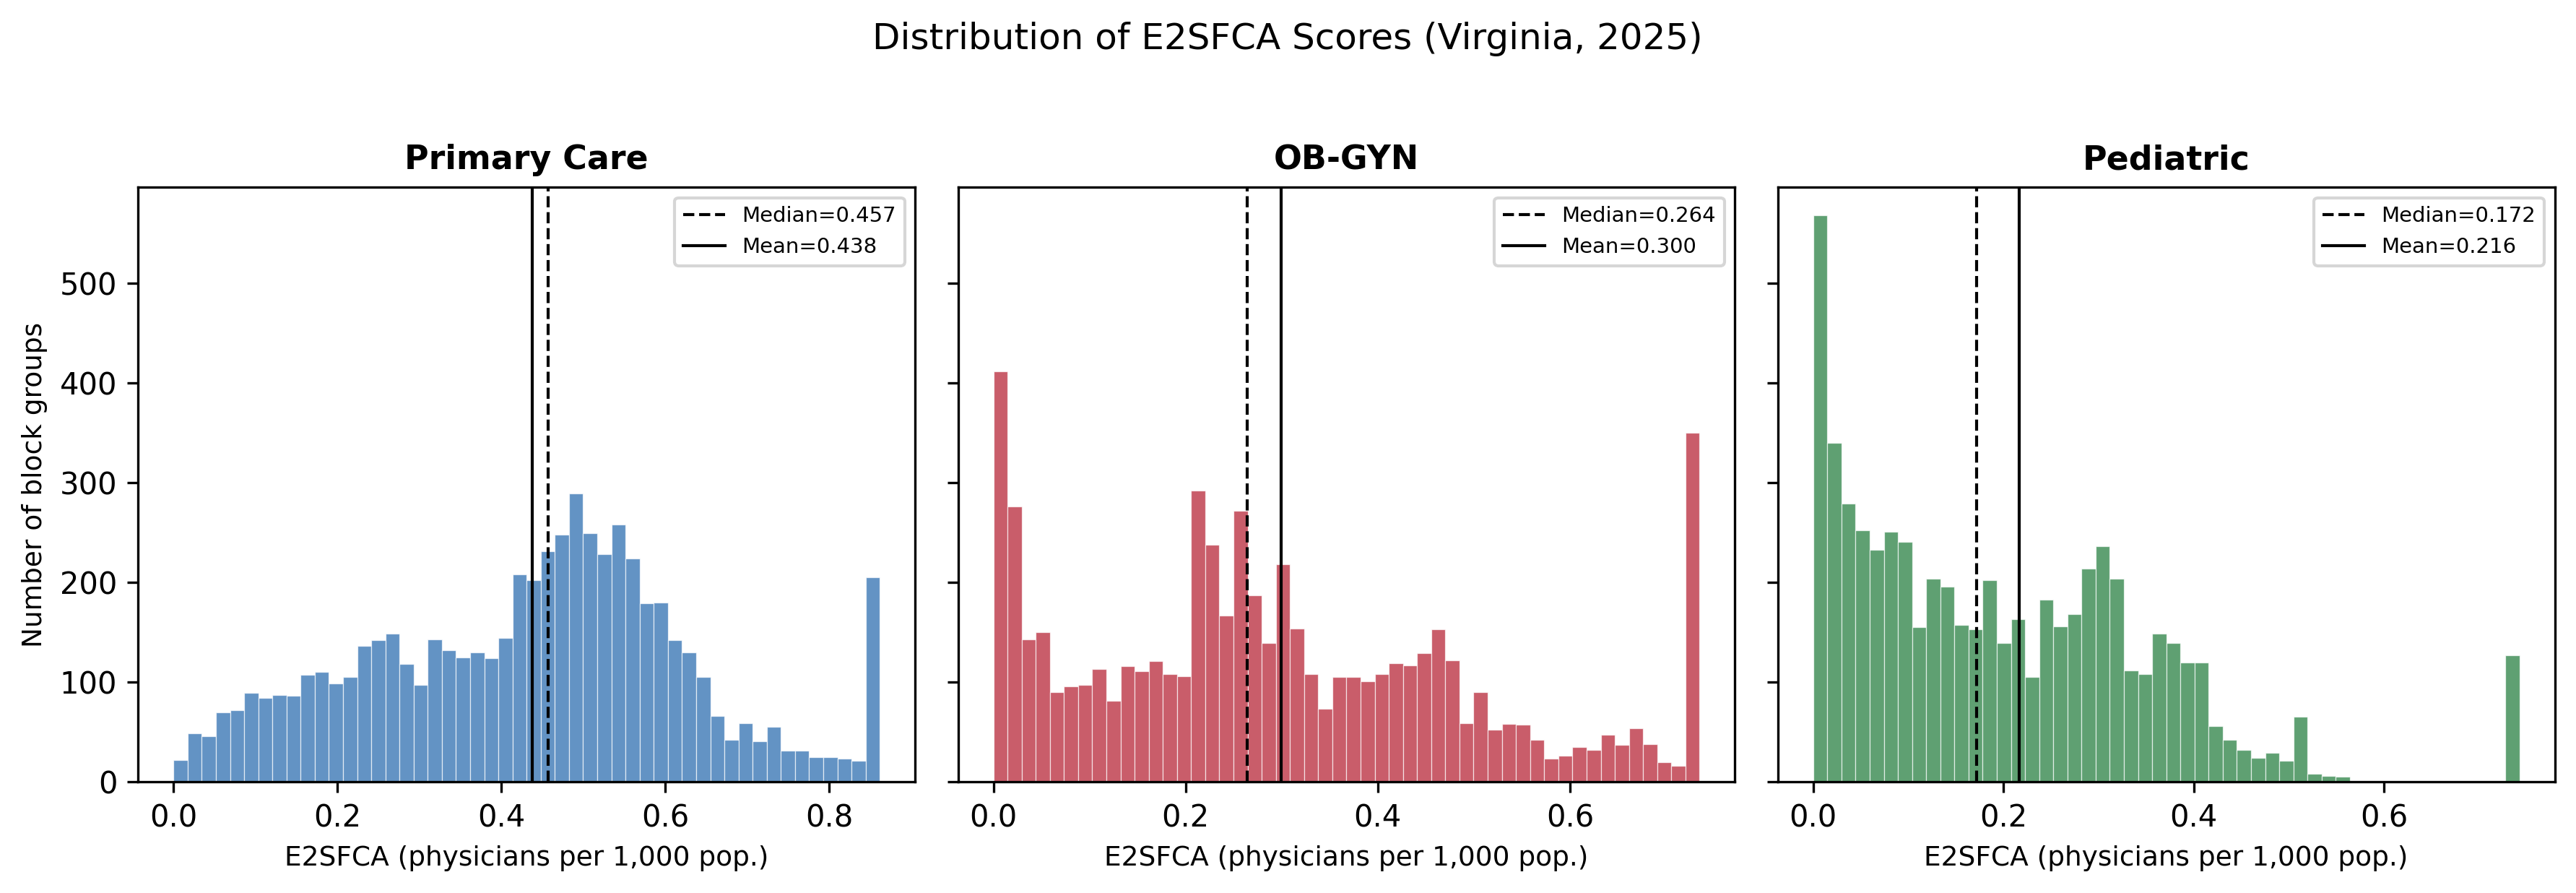
\includegraphics[width=\textwidth]{figures/fig_e2sfca_distribution.png}
\caption{Distribution of E2SFCA scores at the block group level for primary care (left), OB-GYN (center), and pediatrics (right), Virginia, 2025. Dashed vertical lines indicate the median; solid vertical lines indicate the mean. The $x$-axis is truncated at two standard deviations above the mean; values exceeding this threshold are included in the rightmost bin.}
\label{fig:distribution}
\end{figure}

\subsection{Internal consistency}

We verified the arithmetic consistency of the aggregation procedure by comparing county-level provider counts against the sum of block-group-level provider counts within each county. For all three specialties across all 133 Virginia counties in 2022, the discrepancy is zero: the county total exactly equals the sum of its constituent block groups. This check confirms that the spatial join assigning providers to block groups and the subsequent county aggregation introduce no record loss, duplication, or misattribution.

This verification does not test the accuracy of the FCA scores themselves, which depend on the travel time matrix and the Gaussian decay parameters. It confirms only that the input provider data are correctly partitioned across geographic units.

\subsection{Cross-specialty correlation}

If the three datasets measure related aspects of physician accessibility, we would expect moderate positive correlations across specialties. Table~\ref{tab:correlation} reports Spearman rank correlations among the E2SFCA scores at the Virginia block group level in 2022. The strongest correlation is between primary care and OB-GYN ($\rho = 0.694$), followed by primary care and pediatrics ($\rho = 0.515$) and OB-GYN and pediatrics ($\rho = 0.504$). These moderate correlations indicate that areas with better primary care access tend to have better specialist access as well, but with substantial independent variation, consistent with the fact that specialist practices cluster in different locations than primary care offices.

The near\_10\_mean travel time measure shows stronger cross-specialty correlations (primary care to OB-GYN: $\rho = 0.806$; primary care to pediatrics: $\rho = 0.701$; OB-GYN to pediatrics: $\rho = 0.776$). Travel time is driven primarily by the road network and block group remoteness, both of which are shared across specialties, so the higher correlations for this measure are expected.

\begin{table}[ht]
\centering
\caption{Spearman rank correlation matrix of E2SFCA scores and near\_10\_mean travel times across the three physician specialties (Virginia block groups, 2022). All correlations are statistically significant ($p < 0.001$).}
\label{tab:correlation}
\small
\begin{tabular}{lccc}
\toprule
& Primary Care & OB-GYN & Pediatric \\
\midrule
\multicolumn{4}{l}{\textit{E2SFCA scores}} \\
Primary Care & 1.000 & 0.694 & 0.515 \\
OB-GYN & 0.694 & 1.000 & 0.504 \\
Pediatric & 0.515 & 0.504 & 1.000 \\
\midrule
\multicolumn{4}{l}{\textit{Near\_10\_mean travel time}} \\
Primary Care & 1.000 & 0.806 & 0.701 \\
OB-GYN & 0.806 & 1.000 & 0.776 \\
Pediatric & 0.701 & 0.776 & 1.000 \\
\bottomrule
\end{tabular}
\end{table}

\subsection{Temporal consistency}

Multi-year datasets should exhibit high autocorrelation across consecutive years if the underlying spatial distribution of providers changes gradually. We assessed temporal consistency by computing Pearson correlations of E2SFCA scores between consecutive years at the Virginia block group level (Figure~\ref{fig:temporal}).

For primary care, consecutive-year correlations range from 0.919 to 0.956, with one exception: the 2023 to 2024 transition has $r = 0.827$. For pediatrics, consecutive correlations range from 0.914 to 0.982. For OB-GYN, the range is 0.615 to 0.961, with two lower values: 2017 to 2018 ($r = 0.615$) and 2023 to 2024 ($r = 0.768$).

Two patterns warrant explanation. First, the 2023 to 2024 dip appears across all three specialties (primary care $r = 0.827$, OB-GYN $r = 0.768$, pediatrics $r = 0.939$) and coincides with the CMS data expansion described in the Source Data Completeness section. The addition of new enrollment types in 2024 altered the spatial distribution of counted providers, producing a one-time shift in the accessibility surface. Second, the OB-GYN correlation for 2017 to 2018 ($r = 0.615$) is the lowest in the entire series and may reflect early-vintage data quality issues in the CMS file for that specialty.

First-to-last-year correlations provide a measure of long-term structural stability. Primary care has $r = 0.635$ (2018 to 2025), OB-GYN $r = 0.549$ (2017 to 2025), and pediatrics $r = 0.827$ (2018 to 2025). The substantially lower first-to-last correlations for primary care and OB-GYN, relative to pediatrics, reflect the compounding of year-to-year shifts (including the 2024 break). Pediatric access patterns are more spatially stable, likely because pediatric practices are fewer in number and more spatially concentrated in established medical centers.

The 2024 structural break does not invalidate the time series. The pre-2024 years (2018 through 2023) form an internally consistent series, as do the post-expansion years (2024 through 2025). Pooling across the break, however, conflates a data scope change with actual access change. We recommend that users conducting trend analyses either restrict to the pre-2024 period or include the 2024 break as a fixed effect.

\begin{figure}[!htbp]
\centering
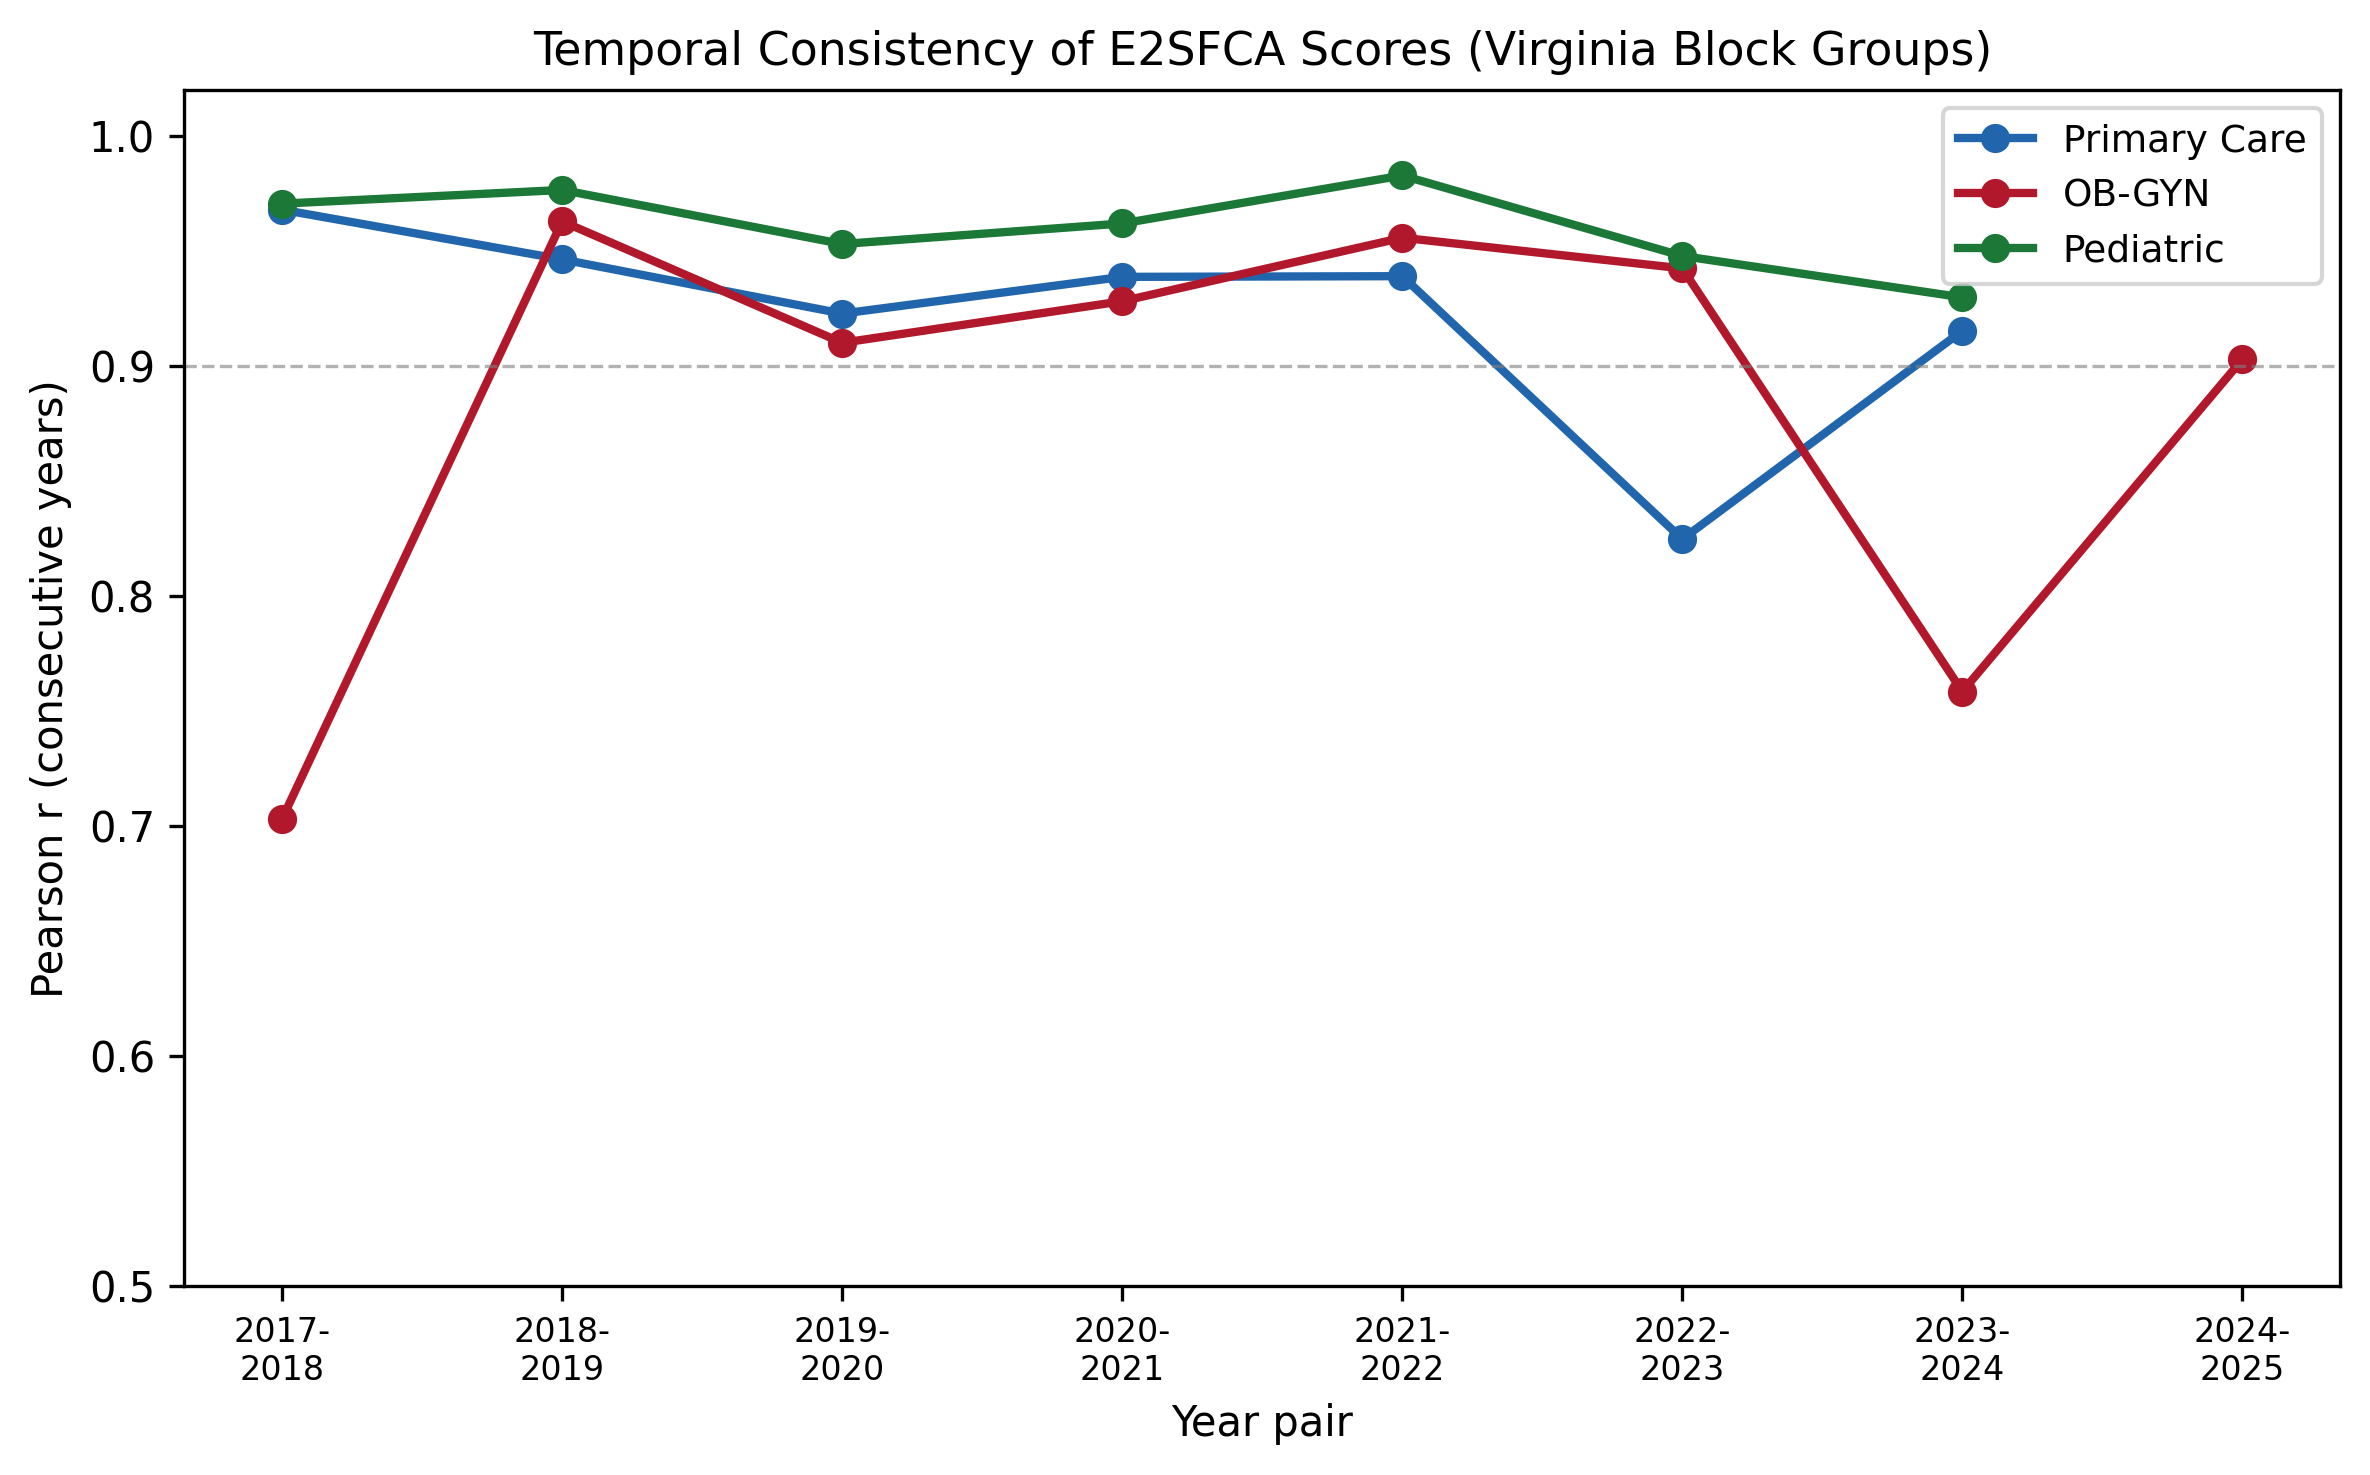
\includegraphics[width=\textwidth]{figures/fig_temporal_consistency.png}
\caption{Temporal consistency of E2SFCA scores: Pearson correlation between consecutive years for each specialty (Virginia block groups). The dashed horizontal line at $r = 0.9$ indicates a reference threshold for high temporal stability. The 2023--2024 dip reflects the CMS data expansion rather than a change in the underlying accessibility surface.}
\label{fig:temporal}
\end{figure}

\subsection{Convergent validity}

To assess whether the E2SFCA scores capture meaningful variation in physician accessibility, we compared them against a simpler measure: the raw count of providers within each county. Unlike the FCA scores, provider counts do not account for population demand, cross-boundary travel, or distance decay; they simply reflect how many physicians have practice addresses in a county.

At the county level in 2022 ($n = 133$ Virginia counties), Spearman rank correlations between the mean E2SFCA score and provider count are: primary care $\rho = 0.608$, OB-GYN $\rho = 0.730$, and pediatrics $\rho = 0.651$ (Figure~\ref{fig:convergent}). The strong rank-order agreement indicates that both measures largely agree on which counties have better or worse access. Pearson linear correlations are weaker: primary care $r = 0.286$, OB-GYN $r = 0.551$, pediatrics $r = 0.533$. The gap between Spearman and Pearson correlations is largest for primary care and reflects a known feature of the FCA methodology: it adjusts for population demand, compressing the distribution relative to raw counts. Counties with large populations (such as Fairfax County) have high provider counts but only moderate FCA scores because those providers serve a correspondingly large population. The weaker linear correlation for primary care, specifically, is consistent with primary care providers being more evenly distributed relative to population than specialists, reducing the variance that the FCA adjustment can explain~\citep{guagliardo2004}.

This divergence is informative: if the FCA scores correlated linearly with raw counts, they would add little information beyond a simple provider census. The FCA's value lies precisely in adjusting for the factors that create divergences: population size, cross-boundary travel, and distance decay.

\begin{figure}[!htbp]
\centering
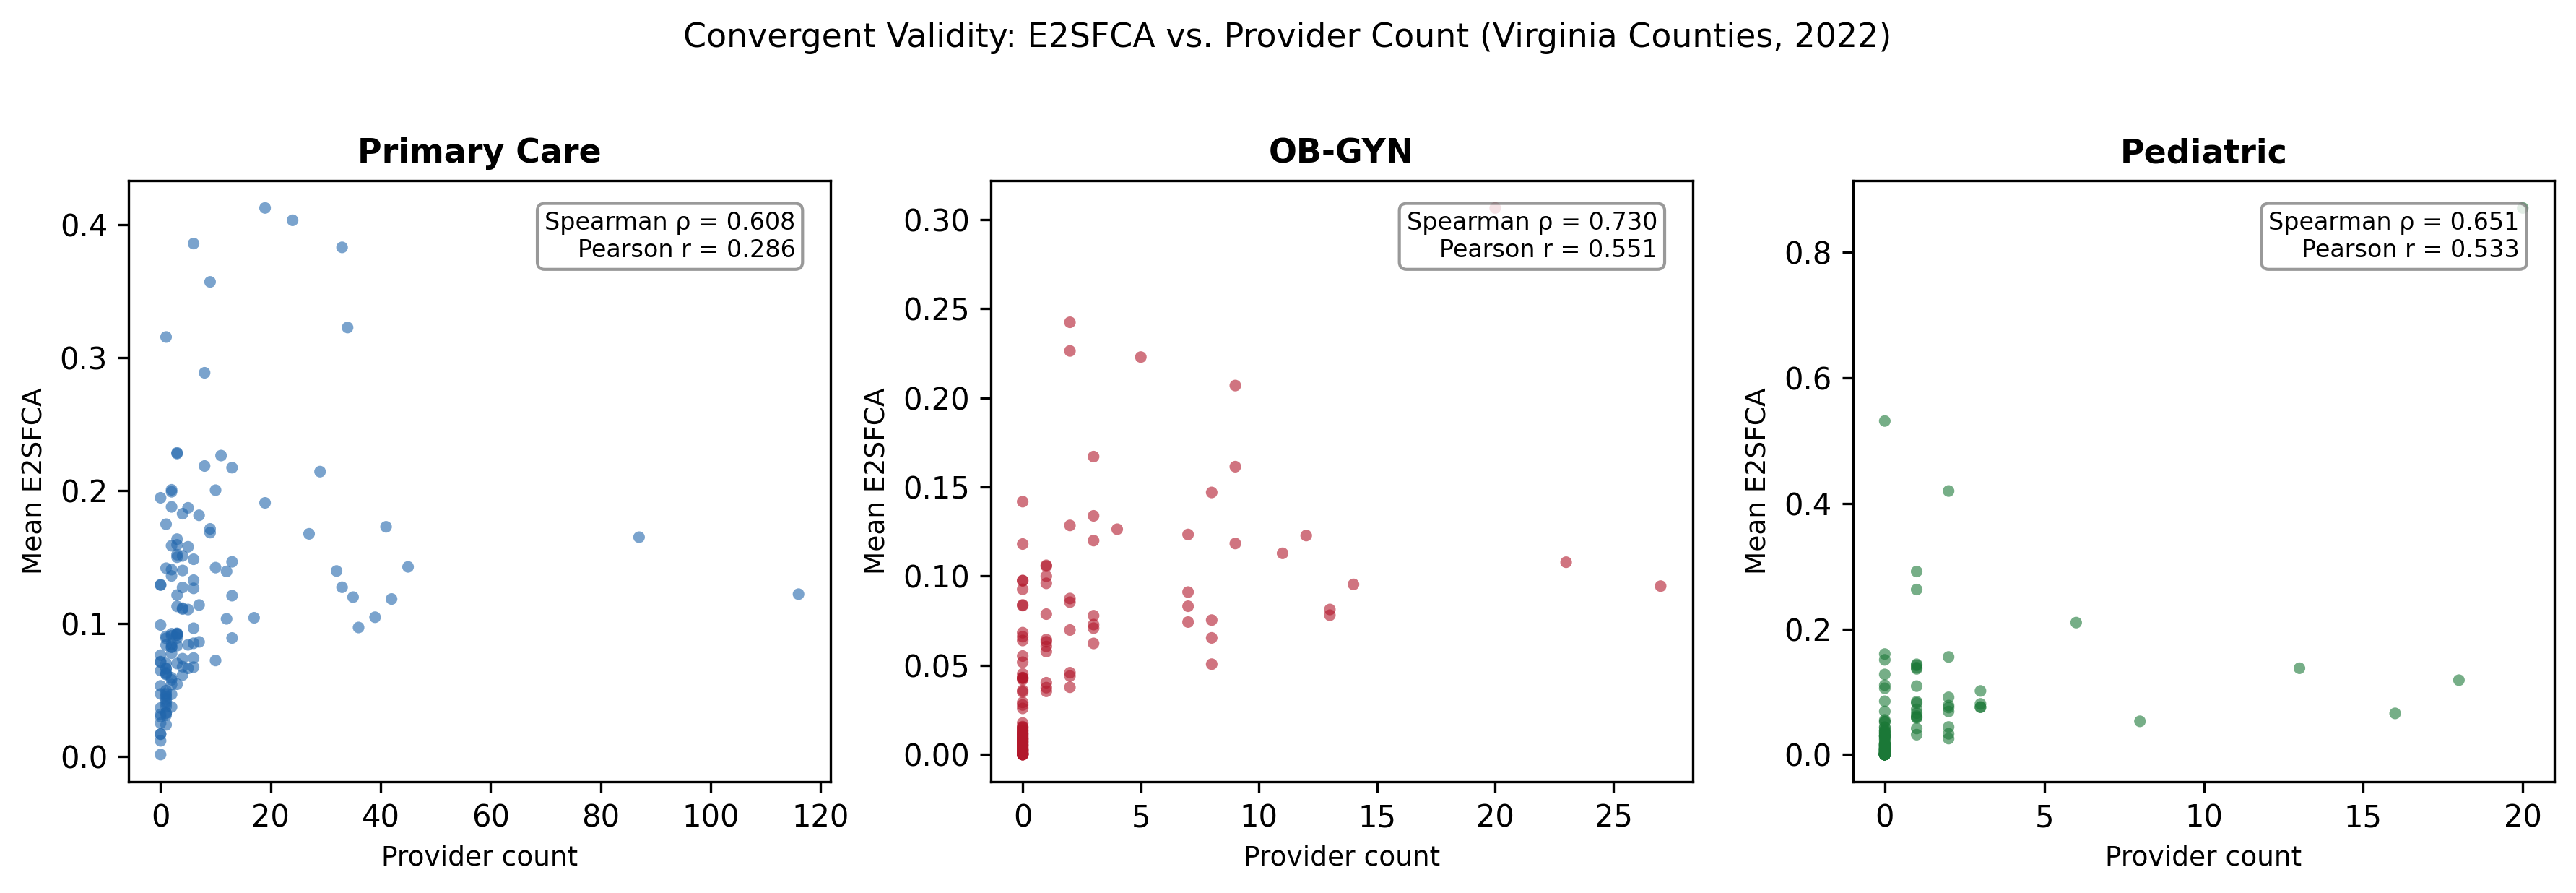
\includegraphics[width=\textwidth]{figures/fig_convergent_validity.png}
\caption{Convergent validity: county-level mean E2SFCA score ($y$-axis) versus raw provider count ($x$-axis) for each specialty (Virginia, 2022, $n = 133$). Spearman ($\rho$) and Pearson ($r$) correlations are annotated. The divergence between rank and linear correlation reflects the FCA adjustment for population demand.}
\label{fig:convergent}
\end{figure}

\subsection{Urban-rural disaggregation}

We classified Virginia block groups into quartiles by county-level provider count and examined mean E2SFCA scores and travel times across these quartiles (2022). For primary care, mean E2SFCA scores increase across quartiles: Q1 = 0.114, Q2 = 0.104, Q3 = 0.134, Q4 = 0.162. Mean travel time to the nearest 10 primary care providers follows the inverse pattern: Q1 = 18.5 minutes, Q2 = 24.6 minutes, Q3 = 21.3 minutes, Q4 = 13.5 minutes (Figure~\ref{fig:urbanrural}). Block groups in the highest provider-count quartile have E2SFCA scores 42\% higher and travel times 27\% shorter than block groups in the lowest quartile.

The non-monotonic pattern in Q2 (which has the lowest FCA score and highest travel time) likely reflects suburban block groups at the fringe of metro areas, where population is high but nearby providers are concentrated in adjacent urban cores. The FCA method captures this pattern, assigning lower scores to high-demand areas whose providers are shared with surrounding block groups. This scenario motivated the original development of FCA methods~\citep{luo2009}, and its appearance in the data supports the face validity of the computed scores.

\begin{figure}[!htbp]
\centering
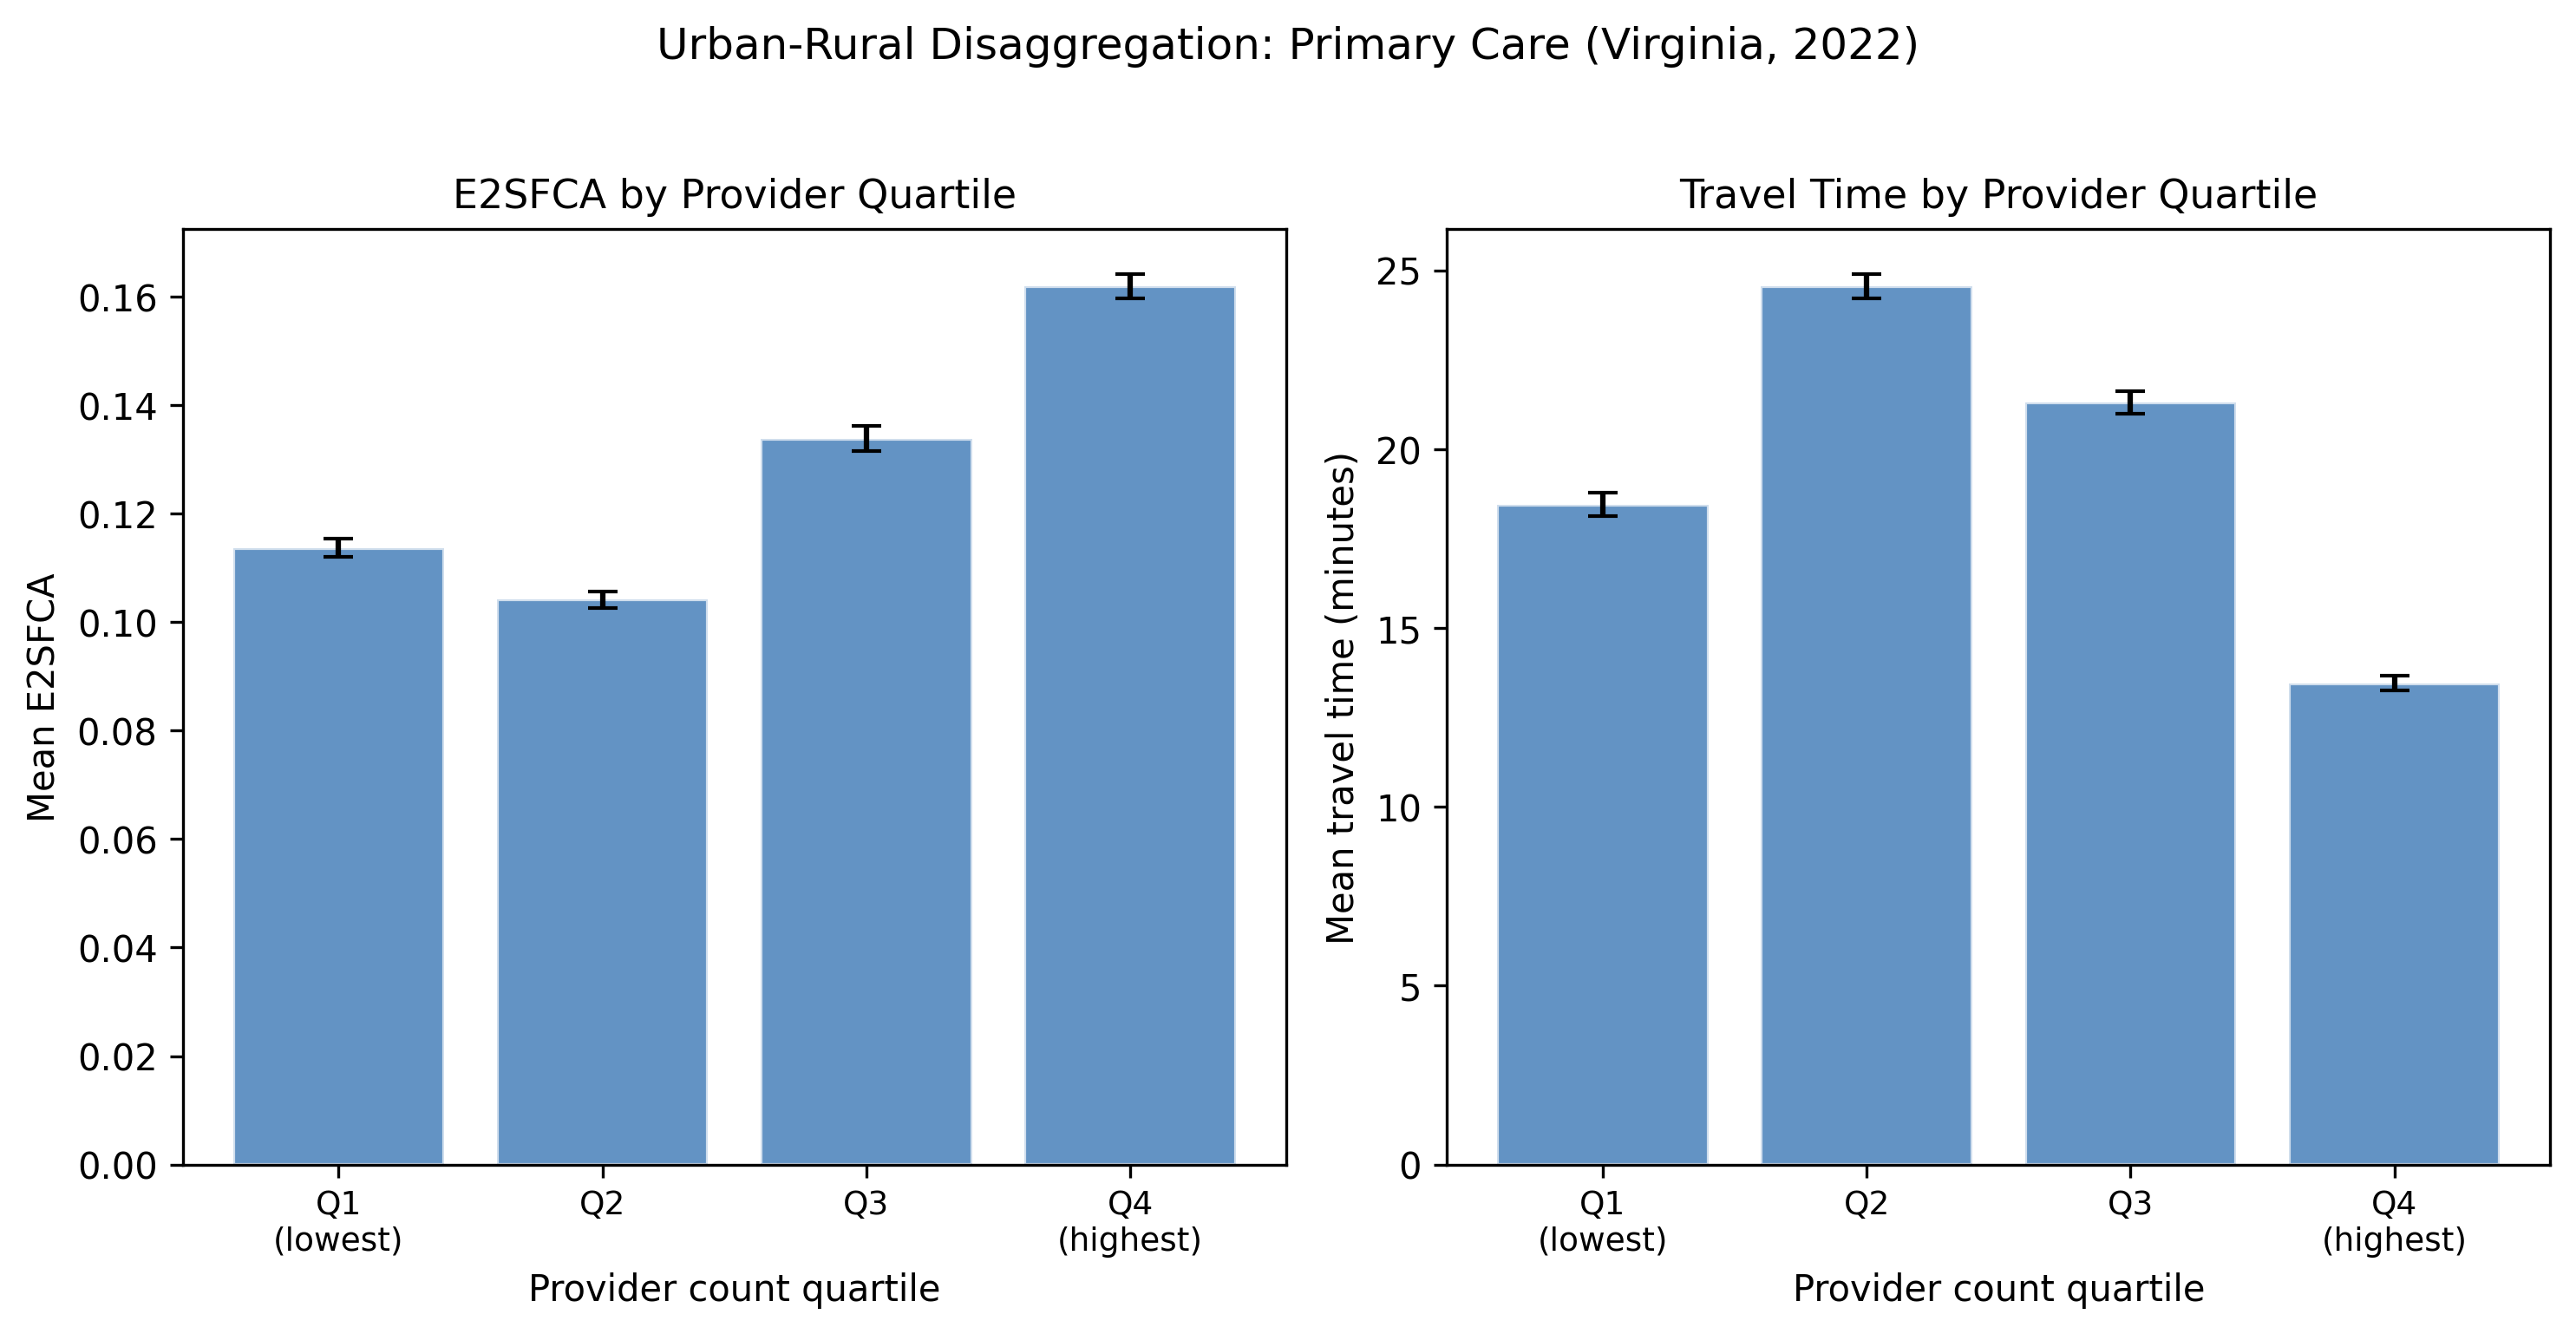
\includegraphics[width=\textwidth]{figures/fig_urban_rural.png}
\caption{Urban-rural disaggregation: mean E2SFCA score (left) and mean travel time to the nearest 10 providers (right) by county-level provider count quartile for primary care (Virginia block groups, 2022). Error bars show one standard error of the mean.}
\label{fig:urbanrural}
\end{figure}

\subsection{Known limitations}

\begin{enumerate}
\item \textbf{CMS enrollment coverage.} The datasets include only physicians enrolled in Medicare, which excludes an estimated 15 to 20 percent of the physician workforce. Physicians who do not participate in Medicare tend to be younger and more concentrated in urban, affluent areas. This omission likely causes a modest underestimation of accessibility in urban block groups relative to rural ones.

\item \textbf{Practice address accuracy.} The CMS file records the address associated with a provider's enrollment record, which may be a billing address, administrative office, or hospital campus rather than the location where patients are seen. This issue is most pronounced for hospital-employed physicians, whose enrollment address may be a central administrative building rather than an outpatient clinic.

\item \textbf{Specialty classification.} Provider specialty is based on CMS enrollment designation, not board certification. Some providers may have changed specialties or hold dual designations. The primary care category (Family Practice, Family Medicine, General Practice) is relatively well-defined, but the OB-GYN and pediatric categories may miss subspecialists whose primary enrollment is in a different category.

\item \textbf{Static road network.} Travel times are computed using OSRM with a free-flow road network from 2020. The calculations do not account for traffic congestion, road closures, seasonal variation, or time-of-day effects. Actual travel times during peak hours in congested urban corridors may be 50 to 100 percent longer than the free-flow estimates.

\item \textbf{Centroid approximation.} Both provider locations and population are assigned to block group centroids, introducing positional uncertainty that is proportional to block group size. In rural western Virginia, block groups can span tens of kilometers, and the centroid may be far from any road or inhabited area. This uncertainty propagates into the FCA scores but does not introduce systematic directional bias.

\item \textbf{ACS margin of error.} The total population denominators carry sampling uncertainty from the ACS 5-year estimates, which is largest at the block group level. This uncertainty is not propagated into the FCA scores. Block groups with very small populations and large margins of error may have FCA scores that are highly sensitive to the population estimate used.

\item \textbf{Fixed Gaussian decay parameter.} The 3SFCA and E2SFCA scores use a single Gaussian scale parameter (20 minutes) applied uniformly across all block groups. Willingness to travel for physician care likely varies with urbanicity, socioeconomic status, and specialty. A spatially varying or specialty-specific decay function may produce different accessibility surfaces, particularly in the transition zones between urban and rural areas~\citep{mcgrail2009}.

\item \textbf{CMS data expansion in 2024.} The addition of new enrollment types to the CMS Doctors and Clinicians file in 2024 roughly tripled primary care provider counts and more than doubled OB-GYN and pediatric counts. This scope change creates a structural break in the time series. Pre-2024 and post-2024 values are not directly comparable without adjustment.

\item \textbf{No provider hours or capacity.} The datasets treat all providers as equal, regardless of whether they practice full-time or part-time. A physician who sees patients one day per week contributes the same to the FCA score as one who practices five days per week. This limitation overstates accessibility in areas served primarily by part-time or locum tenens providers.
\end{enumerate}

%% ============================================================
%% USAGE NOTES
%% ============================================================

\section{Usage Notes}

\subsection{File access and software}

All dataset files are distributed as LZMA-compressed CSV files (\texttt{.csv.xz}). Users can decompress these with standard command-line tools (e.g., \texttt{xz -d} on Linux/macOS) or read them directly in Python using \texttt{pandas.read\_csv()}, which handles \texttt{.csv.xz} files without manual decompression. R users can read the files with \texttt{readr::read\_csv()} or \texttt{data.table::fread()} after decompression. Each file follows a long-format schema with columns for \texttt{geoid}, \texttt{year}, \texttt{measure}, \texttt{value}, \texttt{moe}, \texttt{region\_type}, and \texttt{data\_method}. Files are organized by geographic coverage area (Virginia or NCR) and geographic resolution (block group, tract, county, or health district).

\subsection{Interpreting the measures}

Each specialty produces six measures. The \texttt{cnt} measure reports the raw count of providers within a catchment area. The \texttt{2sfca}, \texttt{e2sfca}, and \texttt{3sfca} measures are floating catchment area (FCA) ratios expressed as physicians per 1{,}000 population, where higher values indicate better spatial access. The three FCA variants differ in how they model distance decay: 2SFCA applies a binary 30-minute threshold, E2SFCA applies stepped distance weights across zones from 0 to 60 minutes, and 3SFCA applies a Gaussian decay function with a scale parameter of 20 minutes. The \texttt{near\_10\_mean} and \texttt{near\_10\_median} measures report the mean and median drive time (in minutes) to the 10 nearest providers, where lower values indicate better access.

Population denominators differ by specialty. Primary care measures use total population, OB-GYN measures use the female population aged 15 and older, and pediatric measures use the population aged 0 to 17. These denominators should be considered when comparing FCA scores across specialties, as the same provider-to-population ratio carries different implications depending on the size and distribution of the relevant demand population.

\subsection{Scope limitations}

The provider data are drawn from the CMS Doctors and Clinicians public use file, which includes only physicians enrolled in the Medicare program. Non-Medicare providers, including those in exclusively private or cash-pay practices, are not captured. This exclusion is most consequential for OB-GYN and pediatric specialties, where a larger share of physicians may serve primarily non-Medicare populations. The geographic scope covers Virginia at block group through health district levels and the National Capital Region at block group through county levels. Areas outside these regions are not included, and border effects may reduce accuracy for census tracts near coverage area boundaries, where residents may access providers located outside the study area.

\subsection{Temporal comparability}

The dataset spans 2018 to 2025 for primary care and pediatric physicians and 2017 to 2025 for OB-GYN physicians. Each CMS data year $t$ is paired with American Community Survey population estimates from year $t-1$, capped at the 2023 ACS vintage for the most recent CMS years. Users should note a structural break in 2024 and 2025: CMS expanded the scope of its public use files in those years, resulting in a sharp increase in provider counts that reflects data coverage changes rather than actual workforce growth. Trend analyses that include 2024 or 2025 should account for this discontinuity, and users should avoid interpreting the increase as evidence of improved provider supply.

\subsection{Current policy use}

These datasets are integrated into two operational public health dashboards: the Virginia Public Health Data dashboard, maintained in partnership with the Virginia Department of Health, and the National Capital Region dashboard. Both platforms present the FCA and distance-based measures alongside other health and demographic indicators for use by public health planners, local governments, and community organizations.

\subsection{Appropriate and inappropriate uses}

The data are well suited for identifying geographic disparities in physician accessibility, comparing access across sub-state regions, and tracking relative changes in provider spatial coverage over time (with attention to the 2024 break). They are also appropriate for use as covariates in regression models examining associations between healthcare access and health outcomes.

The data are not suitable for estimating actual physician utilization, patient volumes, or appointment availability. FCA scores reflect spatial potential for access based on provider locations and population, not realized access. The data should not be used to assess individual physician quality or to compare access across states, as the geographic scope is limited to Virginia and the NCR.

%% ============================================================
%% BACKMATTER
%% ============================================================

\begin{Backmatter}

\paragraph{Acknowledgments}
Initial drafts of individual sections were prepared using Claude (Anthropic), a large language model. All content was reviewed, revised, and validated by the author, who assumes full responsibility for the accuracy and integrity of the final manuscript.

\paragraph{Funding Statement}
Virginia Department of Health, through the Biocomplexity Institute and Initiative at the University of Virginia.

\paragraph{Competing Interests}
The author declares none.

\paragraph{Data Availability Statement}
The datasets described in this paper are deposited on Zenodo under a Creative Commons Attribution 4.0 International license: Primary Care (DOI: \href{https://doi.org/10.5281/zenodo.19152538}{10.5281/zenodo.19152538}), OB-GYN (DOI: \href{https://doi.org/10.5281/zenodo.19152569}{10.5281/zenodo.19152569}), Pediatric (DOI: \href{https://doi.org/10.5281/zenodo.19152601}{10.5281/zenodo.19152601}). Source code is available at \url{https://github.com/uva-bi-sdad/sdc-monorepo}.

\paragraph{Ethical Standards}
This research used only publicly available, de-identified administrative data and does not involve human subjects.

\paragraph{Author Contributions}
A.D.S. designed the study, developed the computational pipeline, performed the technical validation, and wrote the manuscript.

%% ============================================================
%% REFERENCES
%% ============================================================

\begin{thebibliography}{}

\bibitem[AAMC, 2024]{aamc2024}
\textbf{Association of American Medical Colleges (AAMC)} (2024) The Complexities of Physician Supply and Demand: Projections From 2021 to 2036. Washington, DC: AAMC.

\bibitem[Adashi et~al., 2025]{adashi2025}
\textbf{Adashi EY, O'Mahony DP and Gruppuso PA} (2025) The national physician shortage: disconcerting HRSA and AAMC reports. \textit{Journal of General Internal Medicine} \textit{40}(14), 3469--3472.

\bibitem[Andrew et~al., 2024]{andrew2024}
\textbf{Andrew M, Briscombe B, Vardavas R, et~al.} (2024) Identifying strategies for strengthening the health care workforce in the Commonwealth of Virginia. \textit{RAND Health Quarterly} \textit{11}(2), 1.

\bibitem[Atwani et~al., 2025]{atwani2025}
\textbf{Atwani R, Robbins L, Saade G and Kawakita T} (2025) Association of maternity care deserts with maternal and pregnancy-related mortality. \textit{Obstetrics \& Gynecology} \textit{146}(2), 181--188.

\bibitem[Buchalter et~al., 2025]{buchalter2025}
\textbf{Buchalter S, Gunsalus R, Blazel M, et~al.} (2025) Disparities in multi-modal spatial access to primary and specialty care in U.S. neighborhoods. \textit{PLOS ONE} \textit{20}, e0330427.

\bibitem[Congressional Research Service, 2023]{crs2023}
\textbf{Congressional Research Service} (2023) The National Health Service Corps. CRS Report R44970.

\bibitem[Daras et~al., 2019]{daras2019}
\textbf{Daras K, Green MA, Davies A, et~al.} (2019) Open data on health-related neighbourhood features in Great Britain. \textit{Scientific Data} \textit{6}, 107.

\bibitem[Douthit et~al., 2015]{douthit2015}
\textbf{Douthit N, Kiv S, Dwolatzky T and Biswas S} (2015) Exposing some important barriers to health care access in the rural USA. \textit{Public Health} \textit{129}(6), 611--620.

\bibitem[Drescher and Domingue, 2023]{drescher2023}
\textbf{Drescher J and Domingue BW} (2023) The distribution of child physicians and early academic achievement. \textit{Health Services Research} \textit{58}(Suppl 2), 165--174.

\bibitem[Gentili et~al., 2018]{gentili2018}
\textbf{Gentili M, Harati P, Serban N, et~al.} (2018) Quantifying disparities in accessibility and availability of pediatric primary care. \textit{Health Services Research} \textit{53}(3), 1458--1477.

\bibitem[Guagliardo, 2004]{guagliardo2004}
\textbf{Guagliardo MF} (2004) Spatial accessibility of primary care: concepts, methods and challenges. \textit{International Journal of Health Geographics} \textit{3}, 3.

\bibitem[Guagliardo et~al., 2004]{guagliardo2004b}
\textbf{Guagliardo MF, Ronzio CR, Cheung I, et~al.} (2004) Physician accessibility: an urban case study of pediatric providers. \textit{Health \& Place} \textit{10}(3), 273--283.

\bibitem[HRSA, 2024]{hrsa2024}
\textbf{Health Resources and Services Administration (HRSA)} (2024) Designated Health Professional Shortage Areas Statistics.

\bibitem[Kang et~al., 2020]{kang2020}
\textbf{Kang JY, Michels A, Lyu F, et~al.} (2020) Rapidly measuring spatial accessibility of COVID-19 healthcare resources. \textit{International Journal of Health Geographics} \textit{19}, 36.

\bibitem[Koschinsky et~al., 2024]{koschinsky2024}
\textbf{Koschinsky J, Marwell N and Piras G} (2024) Navigating geographical disparities: access to obstetric hospitals in maternity care deserts. \textit{BMC Pregnancy and Childbirth} \textit{24}, 350.

\bibitem[Luo and Wang, 2003]{luo2003}
\textbf{Luo W and Wang F} (2003) Measures of spatial accessibility to health care in a GIS environment. \textit{Environment and Planning B} \textit{30}(6), 865--884.

\bibitem[Luo and Qi, 2009]{luo2009}
\textbf{Luo W and Qi Y} (2009) An enhanced two-step floating catchment area (E2SFCA) method. \textit{Health \& Place} \textit{15}(4), 1100--1107.

\bibitem[March of Dimes, 2024]{marchofdimes2024}
\textbf{Stoneburner A, Lucas R, Fontenot J, et~al.} (2024) Nowhere to Go: Maternity Care Deserts Across the U.S., 2024 Report. March of Dimes.

\bibitem[Marshall et~al., 2017]{marshall2017}
\textbf{Marshall J, Thomas L, Lane NM, et~al.} (2017) Health Disparities in Appalachia. Appalachian Regional Commission.

\bibitem[McGrail and Humphreys, 2009]{mcgrail2009}
\textbf{McGrail MR and Humphreys JS} (2009) Measuring spatial accessibility to primary care in rural areas. \textit{Applied Geography} \textit{29}(4), 533--541.

\bibitem[Penchansky and Thomas, 1981]{penchansky1981}
\textbf{Penchansky R and Thomas JW} (1981) The concept of access: definition and relationship to consumer satisfaction. \textit{Medical Care} \textit{19}(2), 127--140.

\bibitem[Rosenthal et~al., 2005]{rosenthal2005}
\textbf{Rosenthal MB, Zaslavsky A and Newhouse JP} (2005) The geographic distribution of physicians revisited. \textit{Health Services Research} \textit{40}(6), 1931--1952.

\bibitem[Saxena et~al., 2023]{saxena2023}
\textbf{Saxena R, Nagpal BN, Srivastava A, et~al.} (2023) Gravity models for potential spatial healthcare access measurement: a systematic methodological review. \textit{International Journal of Health Geographics} \textit{22}, 30.

\bibitem[Starfield et~al., 2005]{starfield2005}
\textbf{Starfield B, Shi L and Macinko J} (2005) Contribution of primary care to health systems and health. \textit{Milbank Quarterly} \textit{83}(3), 457--502.

\bibitem[Wan et~al., 2012]{wan2012}
\textbf{Wan N, Zou B and Sternberg T} (2012) A three-step floating catchment area method. \textit{International Journal of Geographical Information Science} \textit{26}(6), 1073--1089.

\bibitem[Xia et~al., 2019]{xia2019}
\textbf{Xia Z, Stewart K and Fan J} (2019) Geographic variation in spatial accessibility of U.S. healthcare providers. \textit{PLOS ONE} \textit{14}(4), e0215016.

\end{thebibliography}

\end{Backmatter}

\end{document}
